\documentclass[PICOAPC.tex]{subfiles}

\begin{document}

PICO will set the cosmological paradigm for the 2030's and beyond by measuring the six parameter $\Lambda$CDM with 100,000 more constraining power compared to \planck ; see Figure~\ref{fig:fom} (the improvement between WMAP and Planck was by 100). For an 11-parameter set that include $r$, $\Neff$, and $\Sigma (m_{\nu})$, the improvement is by a factor of $0.5\times10^{9}$. These improvements will test $\Lambda$CDM so stringently that it is hard to imagine it surviving such a scrutiny if it is not fundamentally correct. If tensions deepen to become discrepancies, it would be even more exciting if a new cosmological model emerged. 

%The current host of cosmological observations including the CMB fit within the $\Lambda$CDM model, but they have statistical strength to constrain only six of more than a dozen known cosmological parameters. A figure of merit (FOM) that quantifies the strength of the constraint is the volume of the uncertainty region in the $N$-dimensional parameter space~\citep{core_parameter,Wang2008,pdg2018,Namikawa2010}. 

%Fig.~\ref{fig:fom} shows the increase in the FOM since \cobe\ for the six-parameter $\Lambda$CDM model, as well as for additional cosmological parameters. The Figure only includes data from CMB experiments. The FOM for $\Lambda$CDM improved by a factor of 100 between {\it WMAP} and \planck , and will further improve by a factor of $10^{5}$ with PICO. For the 11-parameter set that includes $\Neff$ shown in the Figure PICO will improve upon \planck\ by a factor of $0.5\times10^{9}$. Having achieved this improvement, there would be only little information left to extract with this parameter set even by a mission with double the resolution and nearly ten times lower noise (Fig.~\ref{fig:fom}). Even stronger FOM improvements are obtained when a 12-parameter set is considered~\citep{picoweb_lcdm}, and when the PICO CMB data will be combined with data sets available in the next decade, including weak lensing, BAO, and cluster of galaxies. 

 \begin{figure}%[t,h]
\hspace{-0.2in}
\parbox{2.7in}{\centerline {
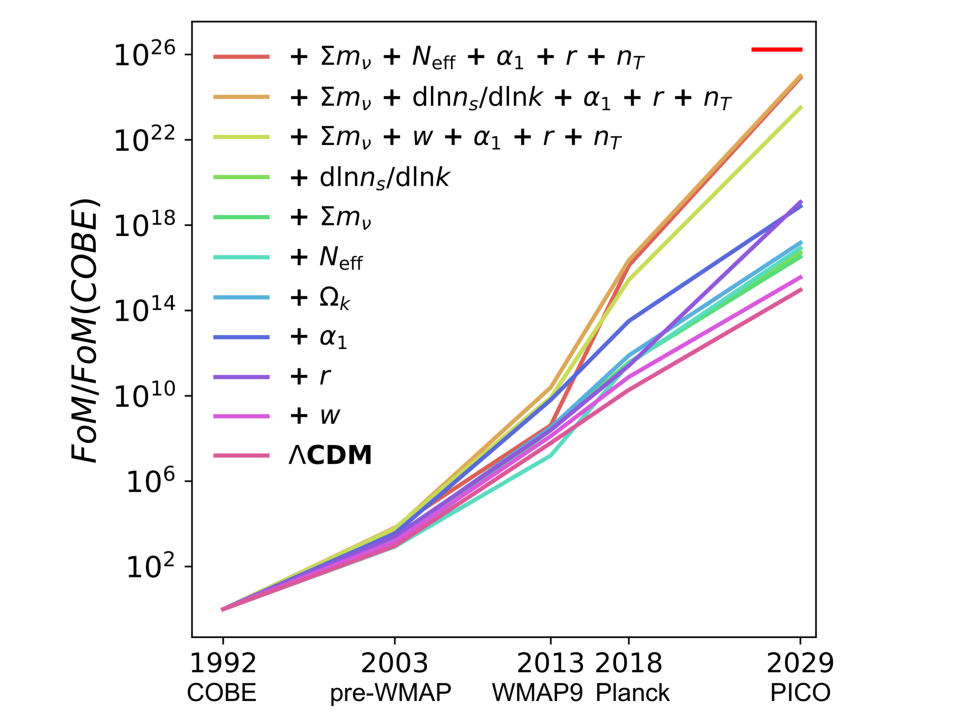
\includegraphics[width=3.0in]{images/fom_plot_CVL+del.pdf} } }
%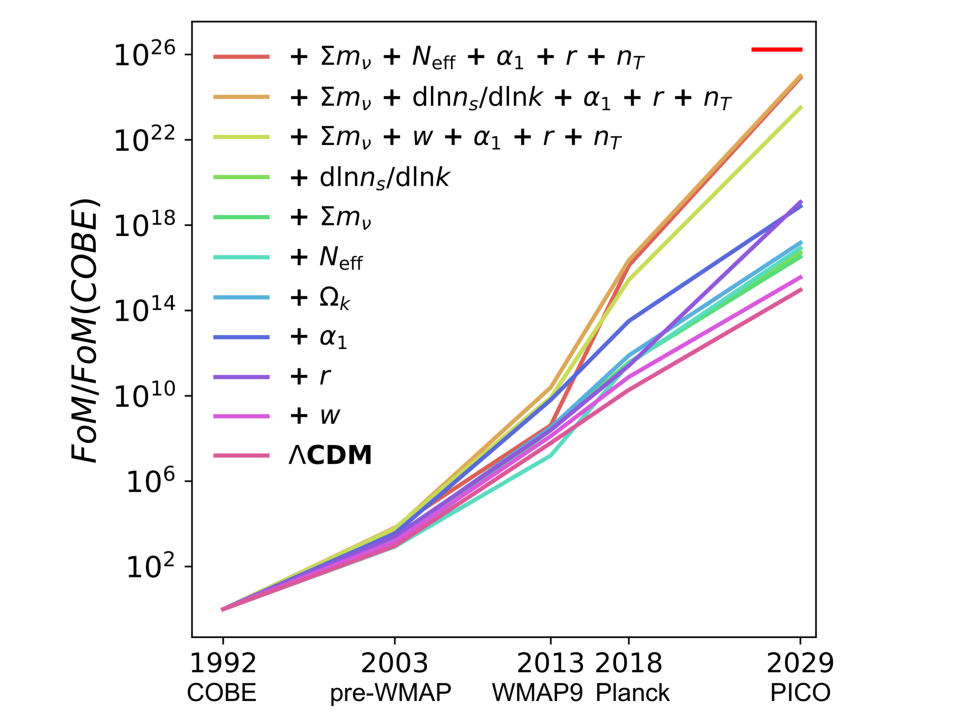
\includegraphics[width=3.0in]{images/fom_plot_CVL+del.pdf} } }
\hspace{0.in}
\parbox{3.8in}{
\caption{\captiontext 
The increase in cosmological parameter constraining power using only CMB data since \cobe . The FoM is the inverse of the uncertainly volume in parameter space. 
%for the $\Lambda$CDM six-parameter model (dark purple) and when adding other cosmological parameters. The FoM Increase in value represents increase in information content. PICO data will continue the average trend (blue line, $\Lambda$CDM + $\alpha_{1}$) of doubling the FOM every 10 months since 1992. 
For an 11-parameter set that includes $\Neff$ (red increasing line) PICO will improve the FoM by a factor of $0.5\times10^{9}$ relative to \planck . It will extract nearly the same information as that attainable by a mission with twice higher resolution and nine times lower noise (top right red horizontal bar), that is, PICO's performance on cosmological parameters is equivalent to that of a `CMB flagship-scale mission'. The constituents of the 11-parameter set are given in~\citet{pico_report}. 
%includes: $w$-dark energy; $r$-the tensor to scalar ratio; $\alpha_{1}$-amplitude of correlated CDM isocurvature perturbations; $\Omega_{k}$-curvature; $\Neff$-effective number of light relics; $\sum m_{\nu}$-sum of neutrino masses; and $d\ln n_{s}/d\ln k$-running of the spectral index.   
\label{fig:fom} } }
\vspace{-0.13in}
\end{figure}

\end{document}


